\documentclass[a4paper]{article} 
\usepackage{graphicx} 
\usepackage[ngerman]{babel} 
\usepackage[ansinew]{inputenc} 
\usepackage[T1]{fontenc} 
\usepackage{tgpagella} 
\usepackage{geometry} 
\usepackage{color} 
\usepackage{microtype} 
\usepackage{minted}
\usepackage{caption}
\usepackage[headsepline,footsepline]{scrpage2}
\usepackage{textcomp}
\usepackage{pdfpages}
\usepackage{mdframed}



\makeatletter
\renewcommand\minted@pygmentize[2][\jobname.pyg]{
  \def\minted@cmd{pygmentize -l #2 -f latex -F tokenmerge
    \minted@opt{gobble} \minted@opt{texcl} \minted@opt{mathescape}
    \minted@opt{startinline} \minted@opt{funcnamehighlighting}
    \minted@opt{linenos} -P "verboptions=\minted@opt{extra}"
    -O encoding=UTF-8,outencoding=iso-8859-1 -o \jobname.out.pyg #1}
  \immediate\write18{\minted@cmd}
  % For debugging, uncomment:
  %\immediate\typeout{\minted@cmd}
  \ifthenelse{\equal{\minted@opt@bgcolor}{}}
   {}
   {\begin{minted@colorbg}{\minted@opt@bgcolor}}
  \input{\jobname.out.pyg}
  \ifthenelse{\equal{\minted@opt@bgcolor}{}}
   {}
   {\end{minted@colorbg}}
  \DeleteFile{\jobname.out.pyg}}
\makeatother


\title{Dokumentation - 6 Übung}
\author{Roman Lumetsberger}
\date{\today}

\newmintedfile[ccode]{cpp}{
               linenos,
               numbersep=5pt,
               frame=lines,
               framesep=2mm
}

\newmintedfile[javacode]{java}{
               linenos,
               numbersep=5pt,
               frame=lines,
               tabsize=2,
               framesep=2mm,
}
\newmintedfile[csscode]{css}{
               linenos,
               numbersep=5pt,
               frame=lines,
               tabsize=2,
               framesep=2mm,
}
\newmintedfile[sqlcode]{sql}{
               linenos,
               numbersep=5pt,
               frame=lines,
               tabsize=2,
               framesep=2mm,
}
\captionsetup{
  font=footnotesize,
  justification=raggedright,
  singlelinecheck=false
}


\newcommand{\srcDir}{../Beispiel/src/at/lumetsnet/caas/}
\newcommand{\testDir}{../Beispiel/test/at/lumetsnet/caas/test/}

\definecolor{lineColor}{RGB}{151,0,0}
\pagestyle{scrheadings}
\clearscrheadfoot
\begin{document}
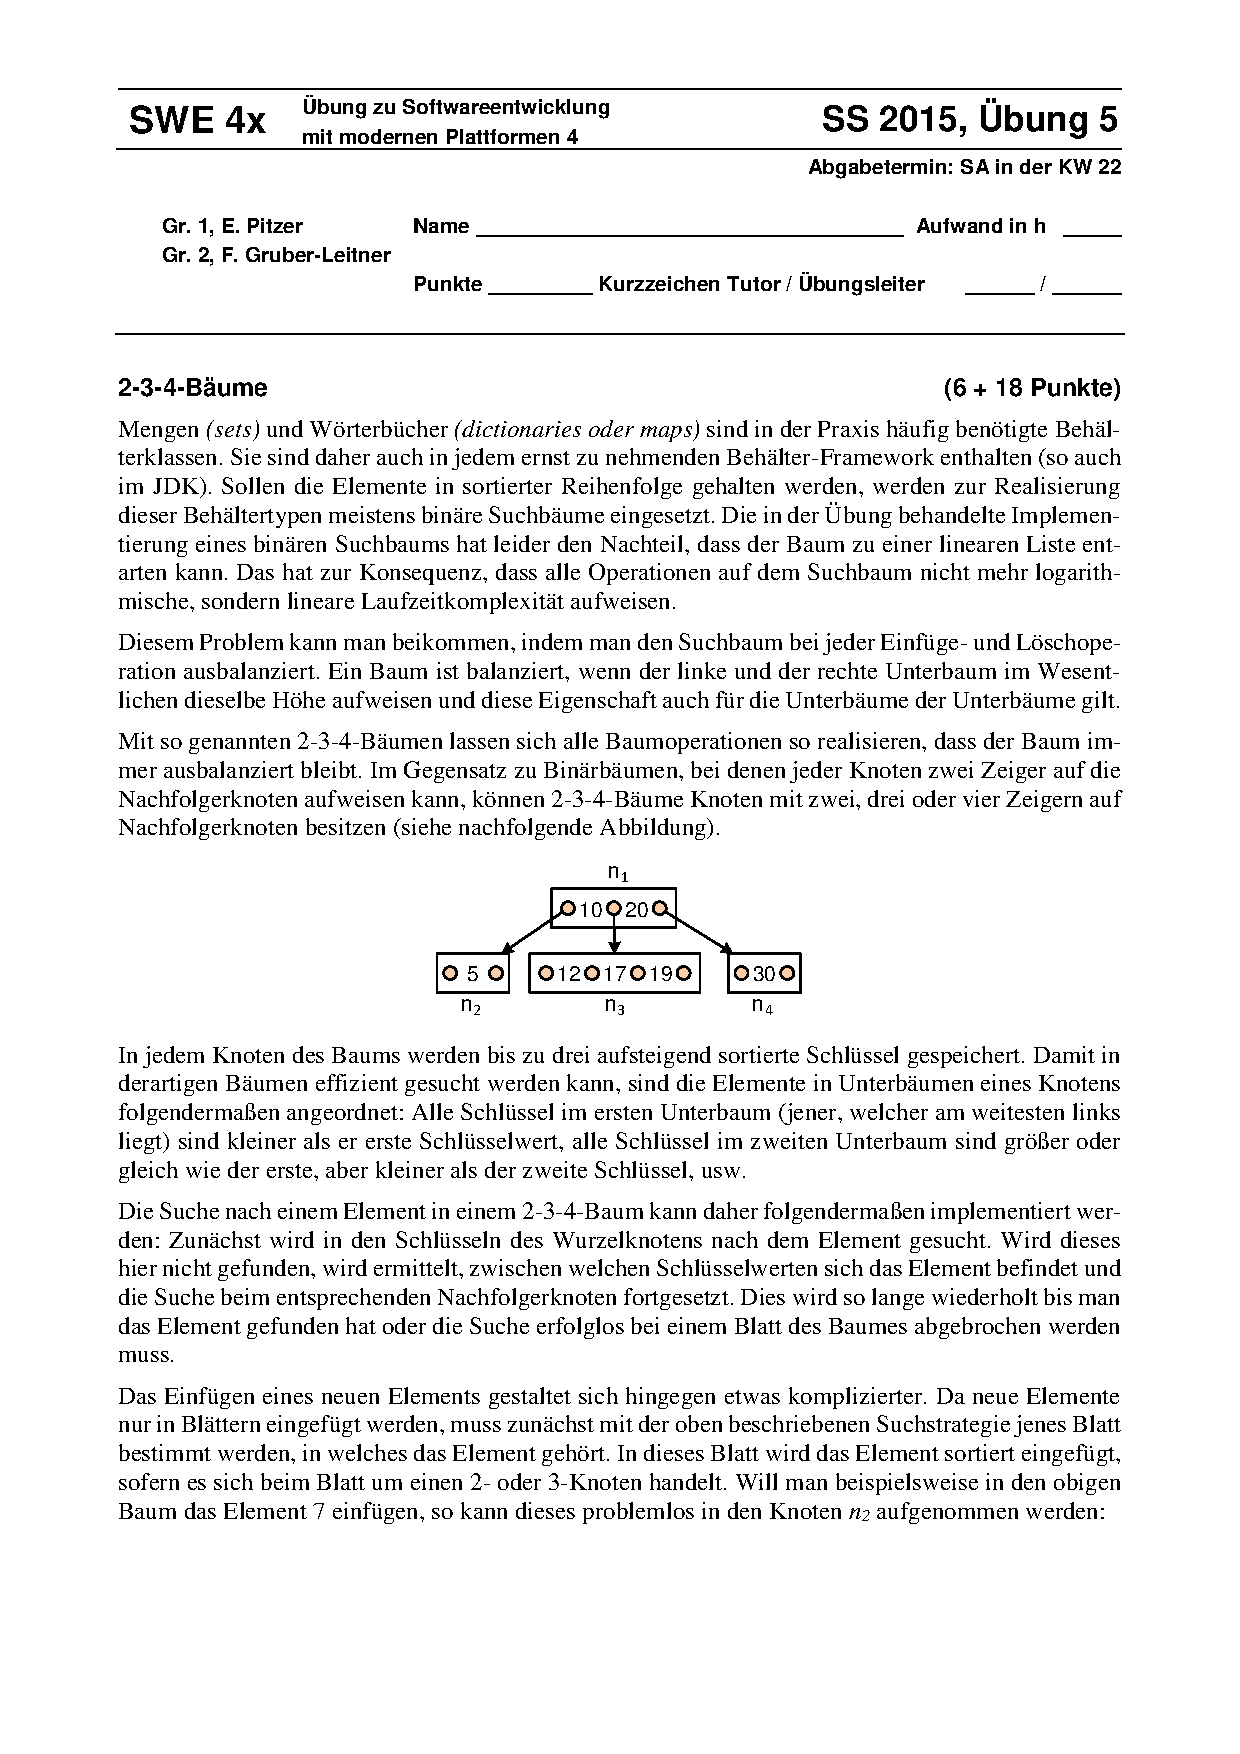
\includepdf[pages=-]{angabe.pdf}

\ihead{SWO3 SS 2015 - �bung 05}
\ifoot{Roman Lumetsberger}
\cfoot{1310307026}
\ofoot{Seite \pagemark}

\section{Bin�re Suchb�ume}
\subsection{L�sungsidee}
F�r die Implementierung des \textit{SortedTreeSet} als bin�ren Suchbaum muss die L�sung der �bung nur um die geforderten Methoden erweitert werden. \newline
Beim Ausf�hren der Testf�lle wurde festgestellt, dass bei gro�en Datenmengen eine \textit{StackOverflowException} geworfen wird. Dies hatte zur Folge, dass die Implementierung der Methode \textit{get} von rekursiv auf iterativ umgebaut werden musste.

\subsubsection{H�he des Baums}
Laut Definition ist die H�he die Anzahl der Kanten von jenem Konten, der am Weitesten von der Wurzel entfernt ist, bis zur Wurzel.
D.h.: 
\begin{itemize}
	\item Ein leerer Baum hat H�he - 1
	\item Ein Baum mit nur einem Knoten hat H�he 0
	\item ...
\end{itemize}
Die H�he des Suchbaums kann gleich beim Einf�gen mitgerechnet werden und erfordert somit keine spezielle Implementierung. \newline

\section{2-3-4 B�ume}
\subsection{L�sungsidee}
Die gruns�tzliche Idee eines \textbf{2-3-4} Baumes ist bereits in der Angabe beschrieben und wird hier nicht mehr extra aufgef�hrt. \newline
Diese Implementierung ben�tigt eine eigene \textit{Node} Klasse, die Datenkomponenten aufnehmen kann. \newline
\begin{itemize}
	\item Liste von Werten (max 3).
	\item Liste der Kindknoten (max 4).
\end{itemize}

\subsubsection{Einf�gen (\textit{add})}
Beim Einf�gen wird der Baum durchlaufen, um ein Blatt zu finden, indem der Wert eingef�gt werden kann. \newline
Dabei wird der Wert immer mit dem in den Knoten gespeicherten Werten verglichen und somit der richtige Kindknoten bestimmt. \newline
Bei dieser Art des Einf�gens in einen \textbf{2-3-4 Baum} ist zu beachten, dass jene Konten, die schon 3 Werte gespeichert haben, gleich beim Besuchen aufgespalten werden.

\subsubsection{Suchen (\textit{get})}
Um einen Wert in einem \textbf{2-3-4 Baum} zu suchen, muss der Baum durchlaufen werden und bei jedem Knoten anhand eines Vergleichs der richtige Kindknoten ermittelt werden.

\subsubsection{Iterator}
Beim \textit{Iterator} m�ssen alle Knoten und deren Werte und Kinder in der korrekten Reihenfolge durchlaufen werden.\newline
Eine einfache M�glichkeit dies zu bewerkstelligen ist es, eine Liste der Werte rekursiv zu ermitteln und dann dessen \textit{Iterator} nach au�en weiterzugben.

\subsubsection{H�he des Baums}
Die H�he des Suchbaums kann auch hier gleich beim Einf�gen mitgerechnet werden und erfordert somit keine spezielle Implementierung. \newline


\pagebreak
\subsection{Sourcecode}

\textbf{SortedSet.java}
\javacode{\srcDir/SortedSet.java}
\textbf{SortedTreeSet.java}
\javacode{\srcDir/SortedTreeSet.java}
\textbf{AbstractSortedTreeSet.java}
\javacode{\srcDir/AbstractSortedTreeSet.java}	
\textbf{BSTSet.java}
\javacode{\srcDir/BSTSet.java}
\textbf{TTFNode.java}
\javacode{\srcDir/TTFNode.java}
\textbf{TwoThreeFourTreeSet.java}
\javacode{\srcDir/TwoThreeFourTreeSet.java}
\textbf{Util.java}
\javacode{\srcDir/Util.java}

\pagebreak
\subsection{Testf�lle}
\begin{mdframed}
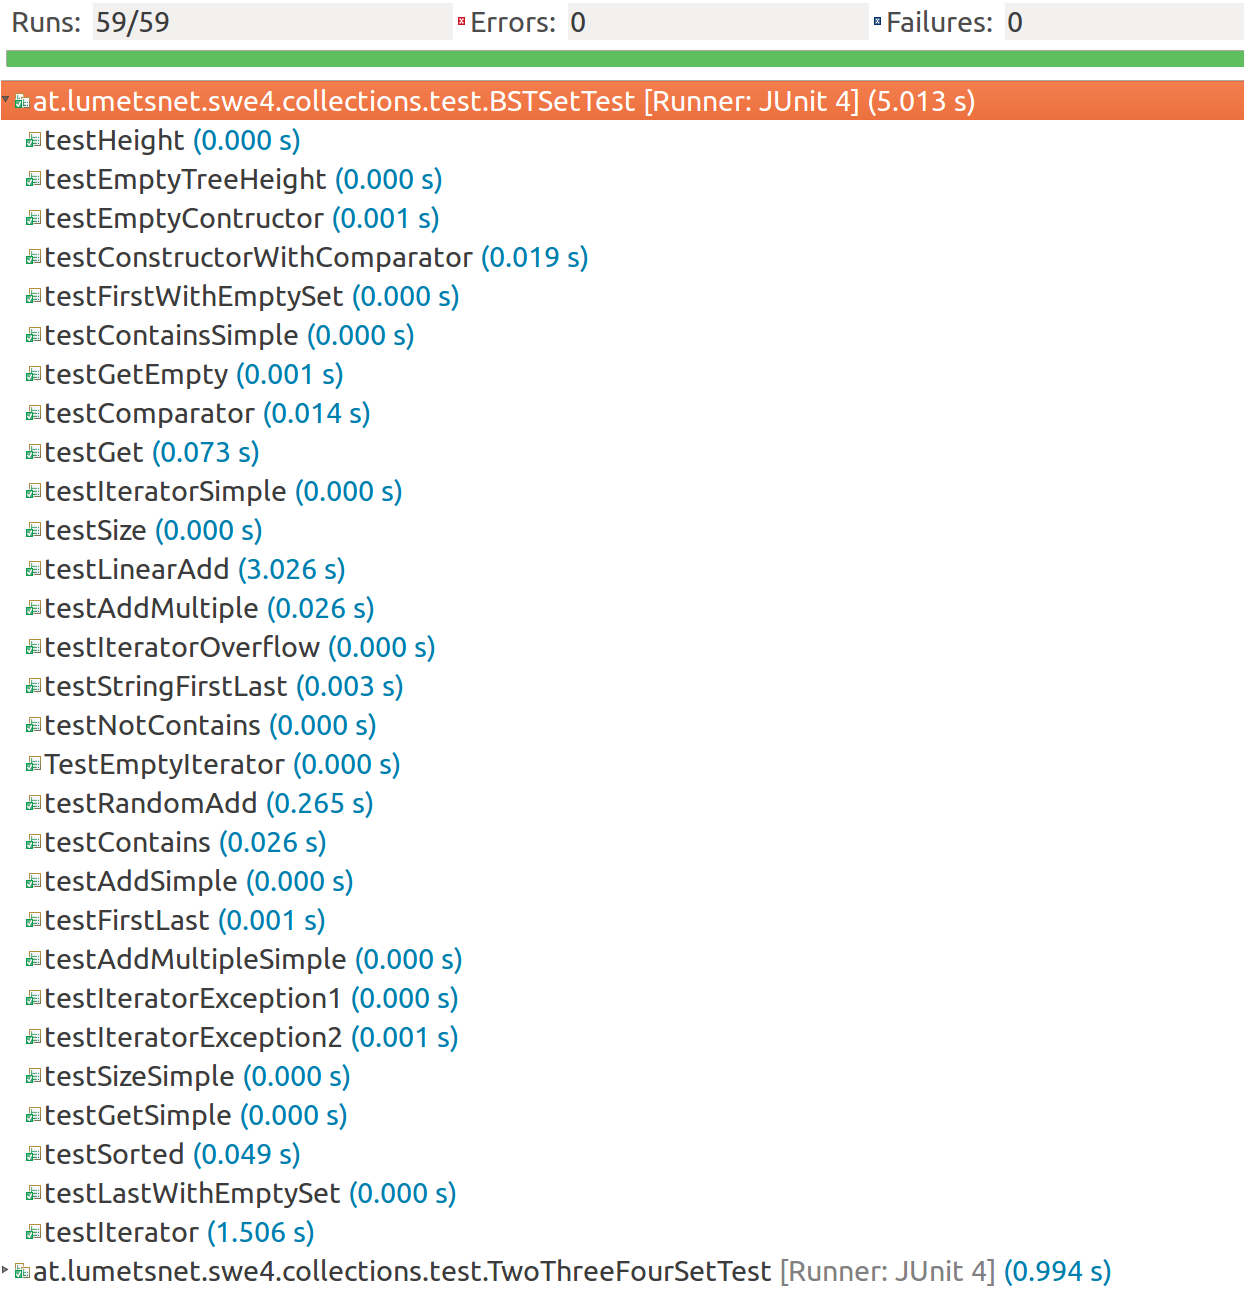
\includegraphics[width=300px]{../Screenshots/1.png}
\end{mdframed}
\begin{mdframed}
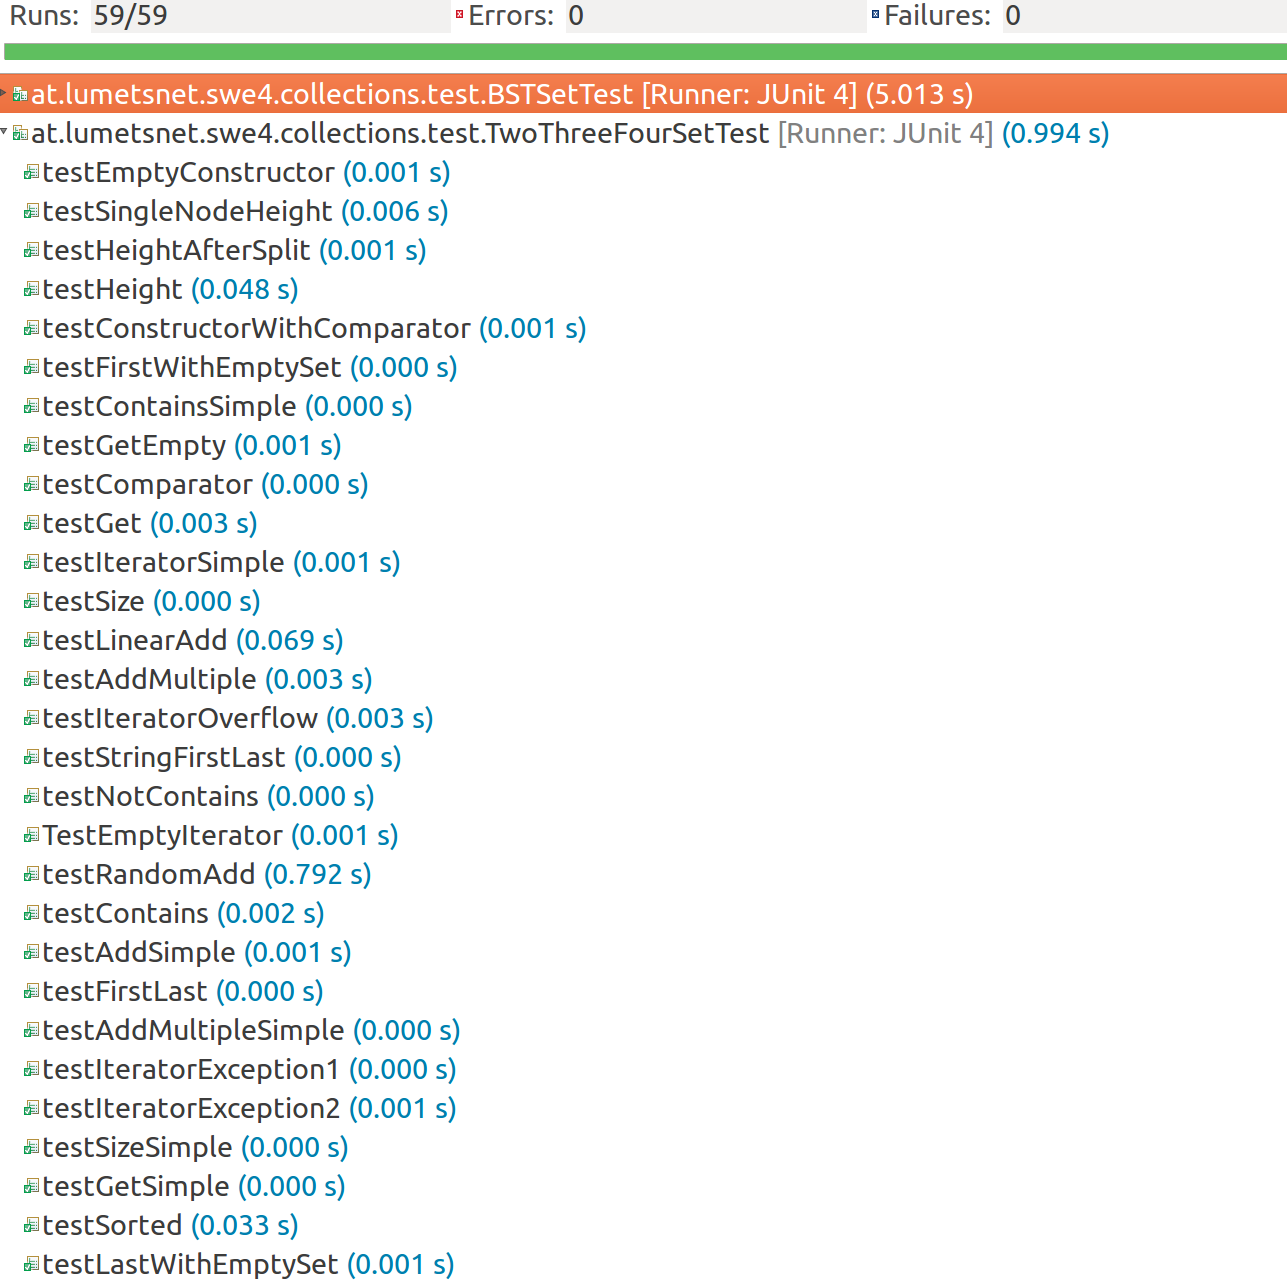
\includegraphics[width=300px]{../Screenshots/2.png}
\end{mdframed}




\end{document}